% (c) 2012-2013 Dimitrios Vrettos - d.vrettos@gmail.com

\chapter{Problemi di I grado in un'incognita}\label{cap:equazioni_I_grado}

\section{Un po' di storia e qualche aneddoto}

Sin dall'antichità l'uomo si è
trovato di fronte a difficoltà pratiche, legate alla vita quotidiana
e ha perciò messo a punto strategie per superarle.

Sembra che nell'antico Egitto le periodiche piene del
Nilo abbiano spinto l'uomo a sviluppare la capacità
di tracciare rette parallele, rette perpendicolari, di misurare il
perimetro e l'area di particolari figure geometriche o
viceversa di calcolare le misure dei lati di poligoni di dato perimetro
o data area per poter ridefinire i confini degli appezzamenti di
terreno.

Il \emph{papiro di Rhind}\footnote{Dal nome dell'inglese A.~H.~Rhind che lo comprò a Luxor nel~1858.}, testo egizio scritto in
ieratico, risalente al~1700~\aC, si autodefinisce
``istruzioni per conoscere tutte le cose
oscure'' e contiene più di~85 problemi con relativi
metodi di soluzione riguardanti il calcolo della capacità di
recipienti e di magazzini, la ricerca dell'area di
appezzamenti di terreno e altre questioni aritmetiche.

Nel problema~24 del papiro, ad esempio, viene calcolato il mucchio
quando esso ed il suo settimo sono uguali a~19. Mucchio è
l'incognita del problema, indicata con il termine
\emph{aha} il cui segno è
% (c) 2012 Dimitrios Vrettos - d.vrettos@gmail.com
\begin{hieroglyph}{\leavevmode \loneSign{{\Hsmaller\Aca GD/66/}}}\end{hieroglyph}.


Noi traduciamo la richiesta nell'equazione~$x+\dfrac{1}{7}x=19$.

Nel~1202 Leonardo Pisano, conosciuto col nome paterno di
``filius Bonacci'' o Fibonacci, pubblicò il
\emph{Liber Abaci} in cui, a partire dall'ottavo
capitolo, presenta vari metodi algebrici per la risoluzione di problemi
di matematica applicata, legati alla realtà
dell'epoca, in particolare
all'ambiente commerciale. I nuovi
``algoritmi'' presentati da Fibonacci,
intendevano facilitare la risoluzione dei problemi di calcolo evitando
l'utilizzo dell'abaco. Nel~1223 a
Pisa, l'imperatore Federico~II di Svevia, assistette a
un singolare torneo tra matematici dell'epoca; il
problema proposto era il seguente:

<<Quante coppie di conigli si ottengono in un anno (salvo i
casi di morte) supponendo che ogni coppia dia alla luce
un'altra coppia ogni mese e che le coppie più
giovani siano in grado di riprodursi già al secondo mese di
vita?>>.

Fibonacci vinse la gara dando al quesito una risposta così rapida da
far persino sospettare che il torneo fosse truccato. La soluzione fu
trovata tramite l'individuazione di una particolare
successione di numeri, nota appunto come successione di Fibonacci.

Secondo la leggenda, il grande matematico Carl Fiedrich Gauss\footnote{matematico, astronomo e fisico tedesco (1777 - 1855).} già
all'età di tre anni avrebbe corretto un errore di
suo padre nel calcolo delle sue finanze. All'età di
10 anni fu autorizzato a seguire le lezioni di aritmetica di un certo
Buttner. Un giorno, agli studenti particolarmente turbolenti, Buttner
diede come compito di punizione il calcolo della somma dei primi~100
numeri naturali, da~1 a~100. Poco dopo, sorprendendo tutti, il giovanissimo Carl
diede la risposta esatta, ``\np{5050}''.
Si era accorto che mettendo in riga tutti i numeri da~1 a~100 e nella
riga sottostante i numeri da~100 a~1, ogni colonna dava come somma~101;
fece dunque il prodotto~$100\times~101$ e divise per~2, ottenendo facilmente il
risultato. Buttner rimase sgomento.

\subsection{Risoluzione dei problemi}

 \epigraph{La risoluzione dei problemi [\ldots] serve ad acuire
 l'ingegno e a dargli la facoltà di penetrare
 l'intera ragione di tutte le cose.}{{\scshape{R. Descartes}}}

I problemi che possono presentarsi nel corso degli studi o
nell'attività lavorativa sono di diversa natura: di
tipo economico, scientifico, sociale, possono riguardare insiemi
numerici o figure geometriche. La matematica ci può aiutare a
risolvere i problemi quando essi possono essere tradotti in
``forma matematica'', quando cioè
è possibile trascrivere in simboli le relazioni che intercorrono
tra le grandezze del problema.

Analizzeremo problemi di tipo algebrico o geometrico, che potranno
essere formalizzati attraverso equazioni di primo grado in una sola
incognita. Prima di buttarci alla risoluzione del problema, procediamo
a:

\begin{enumeratea}
\item una lettura ``attenta'' del
testo al fine di individuare l'ambiente del problema,
le parole chiave, i dati e le informazioni implicite,
l'obiettivo;
\item la scelta della grandezza incognita e la descrizione
dell'insieme in cui si ricerca il suo valore,
ragionando sull'obiettivo del problema (condizioni sull'incognita);
\item la traduzione in ``forma matematica'' delle relazioni che intercorrono tra i
dati e l'obiettivo, cioè l'individuazione dell'equazione risolvente;
\item la risoluzione dell'equazione trovata;
\item il confronto tra la soluzione trovata e le condizioni poste su di essa.
\end{enumeratea}

\begin{problema}
 Un mattone pesa un chilo più mezzo mattone. Quanto pesa un mattone?
\end{problema}

\begin{soluzione}
 La situazione può essere materialmente descritta con nella figura~1.
Togliamo da ogni piatto della bilancia mezzo mattone, la bilancia è
ancora in equilibrio come mostra la figura~2, da ciò possiamo
dedurre che mezzo mattone pesa un chilo. Il mattone intero pesa dunque
due chili.
\begin{center}
 % (c) 2012 Dimitrios Vrettos - d.vrettos@gmail.com
\begin{tikzpicture}[font=\small,x=5mm, y=5mm, scale=.75]

\begin{scope}[fill=black, draw=black]
\filldraw (0,0) rectangle (4,1);
\filldraw[rounded corners=2] (1,1.1)rectangle (3,1.6);
\filldraw (1.8,1.7) rectangle (2.3,8);
\filldraw[rounded corners=2] (1.5,8.1)rectangle (2.6,8.6);
\filldraw (-4,8.7) rectangle (8,9.1);
\filldraw[rounded corners=2] (1.8,8.8)rectangle (2.3,9.8);

\node[name=c1,shape=semicircle,shape border rotate=180, inner sep=3.75mm,draw=black, fill=black] at (-4,3)
{};
\node (a) at (-4,8.7) {};
\draw (a.center)--(c1.arc start);
\draw (a.center)--(c1.arc end);

\node[name=c2,shape=semicircle,shape border rotate=180, inner sep=3.75mm,draw=black, fill=black] at (8,3)
{};
\node (b) at (8,8.7) {};
\draw (b.center)--(c2.arc start);
\draw (b.center)--(c2.arc end);

\filldraw[fill=orange, draw=orange](-5.5,4.02) rectangle (-2.5,5.1);
\filldraw[fill=orange, draw=orange](6.5,4.02) rectangle (8,5.1);
\filldraw[fill=white] (8.3,4) rectangle (9.7,5.1);
\filldraw[fill=white] (8.6,5.1) rectangle (9.4,5.4);
\node () at (9,4.5) {1kg};
\node () at (2,-1) {Figura 1};
\end{scope}

\begin{scope}[fill=black, draw=black, xshift=100mm]
\filldraw (0,0) rectangle (4,1);
\filldraw[rounded corners=2] (1,1.1)rectangle (3,1.6);
\filldraw (1.8,1.7) rectangle (2.3,8);
\filldraw[rounded corners=2] (1.5,8.1)rectangle (2.6,8.6);
\filldraw (-4,8.7) rectangle (8,9.1);
\filldraw[rounded corners=2] (1.8,8.8)rectangle (2.3,9.8);

\node[name=c1,shape=semicircle,shape border rotate=180, inner sep=3.75mm,draw=black, fill=black] at (-4,3)
{};
\node (a) at (-4,8.7) {};
\draw (a.center)--(c1.arc start);
\draw (a.center)--(c1.arc end);

\node[name=c2,shape=semicircle,shape border rotate=180, inner sep=3.75mm,draw=black, fill=black] at (8,3)
{};
\node (b) at (8,8.7) {};
\draw (b.center)--(c2.arc start);
\draw (b.center)--(c2.arc end);

\filldraw[fill=orange, draw=orange](-5,4.02) rectangle (-3,5.1);
\filldraw[fill=white] (7.3,4) rectangle (8.7,5.1);
\filldraw[fill=white] (7.6,5.1) rectangle (8.4,5.4);
\node () at (8,4.5) {1kg};
\node () at (2,-1) {Figura 2};
\end{scope}

\end{tikzpicture}
\end{center}

Risolviamo ora il problema seguendo la procedura sopra suggerita:

\emph{Dati}: peso di un mattone~$=$ peso di mezzo mattone~$+ 1\unit{kg}.$

\emph{Obiettivo}: peso del mattone.

\emph{Procedura risolutiva}:

Come incognita del problema possiamo scegliere il peso del mattone: la
indichiamo con~$p$.
Il valore di~$p$ dovrà essere un numero positivo.
L'equazione risolvente è la traduzione con formalismo
matematico dell'unica relazione contenuta nel testo del
problema:~$p=1+\frac{1}{2}p$.

Risolviamo l'equazione:~$p-\frac{1}{2}p=1\:\Rightarrow\:\frac{1}{2}p=1\:\Rightarrow\: p=2\unit{kg}.$
La soluzione ottenuta è accettabile; il problema è determinato.
\end{soluzione}

\begin{problema}
 Aggiungendo ad un numero naturale i suoi tre quarti, si ottiene il suo
doppio aumentato di~10. Qual è il numero?
\end{problema}

\begin{soluzione}
L'ambiente del problema è numerico: si cerca un numero
naturale. Indichiamo con~$n$ l'incognita
cerchiamo quindi~$n\in\insN$. La lettura attenta del testo mette
in luce le operazioni che dobbiamo eseguire
sull'incognita e che traduciamo nei dati:

\emph{Dati}:~$n+\dfrac{3}{4}n=2n+10$.

\emph{Obiettivo}:~$n\in\insN$.

\emph{Procedura risolutiva}:

L'equazione risolvente è già indicata nei dati~$n+\dfrac{3}{4}n=2n+10$.

Per risolverla moltiplichiamo ambo i membri per~4, otteniamo:
\[4n+3n-8n=40\quad\Rightarrow\quad -n=40\quad\Rightarrow\quad n=-40.\]

La soluzione non è accettabile per le condizioni poste; il problema
non ha soluzione.
\end{soluzione}

\begin{problema}
 Il~1{\textdegree} gennaio~1990 Chiara aveva il doppio
dell'età di Aldo; il~1{\textdegree} gennaio~2000
Chiara aveva vent'anni più di Aldo. Qual era
l'età di Chiara il~1{\textdegree} gennaio~2010?
\end{problema}

\begin{soluzione}
Leggendo attentamente il problema notiamo che le incognite sono due:
l'età di Chiara e l'età di Aldo.
Indichiamo perciò con~$c$ l'età di
Chiara al~1990 e con~$a$ quella di Aldo.

Nel~2000 la loro età sarà aumentata di~10 anni. Naturalmente la
soluzione del problema sarà nell'insieme dei numeri
naturali. Scriviamo dati e obiettivo usando il formalismo matematico:

\emph{Dati}: nel~1990:~$c=2a$, nel~2000:~$c+10=(a+10)+20$.

\emph{Obiettivo}: L'età di Chiara nel~2010.

\emph{Procedura risolutiva}:
Osserviamo che una volta determinata l'età di Chiara
nel~1990, basterà aggiungere a questa~20 per ottenere la soluzione,
pertanto l'età di Chiara nel~2010 è~$c+20$.
Trasformiamo la seconda relazione riportata nei dati sostituendo
l'informazione relativa al~1990,
si ottiene~$2a+10=a+10+20\Rightarrow 2a-a=20\Rightarrow a=20$.
L'età di Aldo nel~1990 era~20, quindi~$c=40$.
Dunque, l'età di Chiara nel~2010 era~$c+20=40+20=60$.
La soluzione è accettabile; il problema è determinato.
\end{soluzione}

\begin{problema}
 Calcolare l'area di un rettangolo in cui
l'altezza supera $\dfrac{1}{3}$ della base di~8m e il
perimetro è~$\dfrac{20}{7}$ della base stessa.
\end{problema}

\begin{soluzione}
 Il problema è di tipo geometrico e riguarda un rettangolo. Facendo riferimento alla figura abbiamo:
\begin{multicols}{2}
 \emph{Dati}:~$\overline{AD}=\dfrac{1}{3}\overline{AB}+8$, $\quad 2p=\dfrac{20}{7}\overline{AB}$.

\emph{Obiettivo}: L'$\Area (ABCD).$

\begin{center}
 % (c) 2012 Dimitrios Vrettos - d.vrettos@gmail.com
\begin{tikzpicture}[font=\small,x=8mm, y=3.5mm]

\draw (0,0) rectangle (4,4);

\begin{scope}[left]
\node  at (0,4) {$A$};
\node  at (0,0) {$D$};
\end{scope}

\begin{scope}[right]
\node  at (4,4) {$B$};
\node  at (4,0) {$C$};
\end{scope}
\end{tikzpicture}
\end{center}
\end{multicols}

\emph{Procedura risolutiva}:
$\Area (ABCD)=\text{ misura base }\cdot \text{ misura altezza }=\overline{AB}\cdot \overline{AD}$.

Dobbiamo dunque determinare queste due misure. I dati del problema
indicano che la misura dell'altezza dipende da quella
della base; una volta trovata questa misura basta farne un terzo e
aggiungere~8 per avere quella dell'altezza; questo
ragionamento ci fa scegliere come incognita~$\overline{AB}=x$
con~$x$ numero reale positivo.

Traduciamo con formalismo matematico la prima e la seconda relazione
contenuta nei dati:
$\overline{AD}=\dfrac{1}{3}x+8$ e~$2p=\dfrac{20}{7}x$.

Sappiamo che il perimetro di un rettangolo è il doppio della somma
della base con l'altezza. Riscriviamo con linguaggio
matematico anche questa relazione:~$2\cdot \left(x+\dfrac{1}{3}x+8\right)=\dfrac{20}{7}x$
che risulta l'equazione risolvente.

Svolgiamo i calcoli e otteniamo~$4x=21\cdot 16\Rightarrow x=84\Rightarrow\overline{AB}=84$ e quindi~$\overline{AD}=36$.
Ottenute le misure della base e dell'altezza calcoliamo~$\Area (ABCD)=36\cdot 84=\np[m^2]{3024}$.
\end{soluzione}

\begin{problema}
In un triangolo rettangolo il perimetro è~$120\unit{cm}$ e un cateto è~$3/5$
dell'ipotenusa. Determinare l'area del
triangolo.
\end{problema}

\begin{soluzione}
 Il problema è di tipo geometrico e riguarda un triangolo rettangolo.
Rappresentiamo il triangolo:

\begin{multicols}{2}

\emph{Dati}:~$C\hat{A}B=$ angolo retto, $2p= 120$, $\overline{AC}=\dfrac{3}{5}\overline{CB}$.

\emph{Obiettivo}: L'$\Area (ABC)$.
\begin{center}
 % (c) 2012 Dimitrios Vrettos - d.vrettos@gmail.com
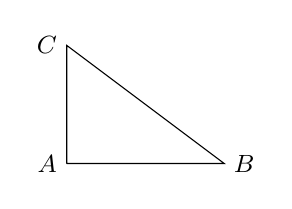
\begin{tikzpicture}[font=\small,x=5mm, y=5mm]

\draw (0,0)-- (4,0)--(0,3)--(0,0);

 \begin{scope}[left]
\node  at (0,3) {$C$};
\node  at (0,0) {$A$};
\end{scope}

\node[right]  at (4,0) {$B$};

\end{tikzpicture}
\end{center}
\end{multicols}



\emph{Procedura risolutiva}:~$\Area (ABC) =\dfrac{1}{2}\overline{AB}\cdot \overline{AC}$.

Per calcolare l'area, occorre determinare la misura dei
cateti del triangolo rettangolo; i dati del problema ci danno una
relazione tra la misura di un cateto e la misura
dell'ipotenusa; conosciamo anche il perimetro del
triangolo.

Scegliamo come incognita la misura in cm di~$\overline{CB}$, cioè
$\overline{CB}=x$ con~$x\in\insR^{+}$.

\emph{Formalizziamo i dati}:
 \begin{equation}\label{14.1}
 \overline{CB} =x;\quad \overline{AC} =\dfrac{3}{5}x;\quad \overline{AB} +x+\dfrac{3}{5}x=120.
 \end{equation}


Per poter scrivere un'equazione che ci permetta di determinare il
valore dell'incognita ci manca la misura di $\overline{AB}$. Sembra
che il problema sia privo di un'informazione. Tuttavia, il triangolo
dato è rettangolo, quindi tra i suoi lati sussiste la relazione del
teorema di Pitagora:
$\overline {CB}^{2}=\overline {AB}^{2}+\overline {AC}^{2}$.

Pertanto possiamo determinare la misura di~$\overline{AB}$:
\[\overline{AB}=\sqrt{\overline{CB}^{2}-\overline {AC}^{2}}=\sqrt{x^{2}-\left(\frac{3}{5}x\right)^{2}}=\sqrt{\frac{16}{25}x^{2}}=\frac{4}{5}x.\]

Con questo dato riscriviamo la \ref{14.1} che risulta essere
l'equazione risolvente del problema
\[\frac{4}{5}x+x+\dfrac{3}{5}x=120\quad\Rightarrow\quad 12x=120\cdot 5\quad\Rightarrow\quad x=50\quad\Rightarrow\quad\overline{CB}=50.\]

Quindi~$\overline {AC} = 30\unit{cm}$ e~$\overline {AB}= 40\unit{cm}\quad\Rightarrow\quad\Area (ABC)=\dfrac{30\cdot 40}{2}=600\unit{cm}^{2}$.
\end{soluzione}

\newpage
% (c) 2012 Silvia Cibola - silvia.cibola@gmail.com
% (c) 2012-2014 Dimitrios Vrettos - d.vrettos@gmail.com

Gli esercizi indicati con (\croce) sono tratti da \emph{Matematica~1}, Dipartimento di Matematica, ITIS V.~Volterra, San Donà di Piave, Versione [11-12][S-A11], pg.~90;
licenza CC,BY-NC-BD, per gentile concessione dei professori che hanno redatto il libro.
%Il libro è scaricabile da \url{http://www.istitutovolterra.it/dipartimenti/matematica/dipmath/docs/M1_1112.pdf}

\section{Esercizi}
\subsection{Problemi con i numeri}
\begin{multicols}{2}
\begin{esercizio}[\Ast]
Determina due numeri, sapendo che la loro somma vale~$70$ e il secondo supera di~$16$ il doppio del primo.
\end{esercizio}

\begin{esercizio}[\Ast]
Determina due numeri, sapendo che il secondo supera di~$17$ il triplo del primo e che la loro somma è~$101$.
\end{esercizio}

\begin{esercizio}[\Ast]
Determinare due numeri dispari consecutivi sapendo che il minore supera di~$10$ i~$\frac{3}{7}$ del maggiore.
\end{esercizio}

\begin{esercizio}[\Ast]
Sommando~$15$ al doppio di un numero si ottengono i~$\frac{7}{2}$ del numero stesso. Qual è il numero?
\end{esercizio}

\begin{esercizio}
Determinare due numeri consecutivi sapendo che i~$\frac{4}{9}$ del maggiore superano di~$8$ i~$\frac{2}{13}$ del minore.
\end{esercizio}

\begin{esercizio}[\Ast]
Se ad un numero sommiamo il suo doppio, il suo triplo, il suo quintuplo e sottraiamo~$21$, otteniamo~$100$. Qual è il numero?
\end{esercizio}

\begin{esercizio}[\Ast]
Trova il prodotto tra due numeri, sapendo che: se al primo numero sottraiamo~$50$ otteniamo~$50$ meno il primo numero; se al doppio del secondo aggiungiamo il suo consecutivo, otteniamo~$151$.
\end{esercizio}

\begin{esercizio}[\Ast]
Se a~$\frac{1}{25}$ sottraiamo un numero, otteniamo la quinta parte del numero stesso. Qual è questo numero?
\end{esercizio}

\begin{esercizio}[\Ast]
Carlo ha~$152$ caramelle e vuole dividerle con le sue due sorelline. Quante caramelle resteranno a Carlo se le ha distribuite in modo che ogni sorellina ne abbia la metà delle sue?
\end{esercizio}

\begin{esercizio}[\Ast]
Se a~$\frac{5}{2}$ sottraiamo un numero, otteniamo il numero stesso aumentato di~$\frac{2}{3}$. Di quale numero si tratta?
\end{esercizio}

\begin{esercizio}[\Ast]
Se ad un numero sottraiamo~$34$ e sommiamo~$75$, otteniamo~$200$. Qual è il numero?
\end{esercizio}

\begin{esercizio}[\Ast]
Se alla terza parte di un numero sommiamo~$45$ e poi sottraiamo~$15$, otteniamo~$45$. Qual è il numero?
\end{esercizio}

\begin{esercizio}[\Ast]
Se ad un numero sommiamo il doppio del suo consecutivo otteniamo~$77$. Qual è il numero?
\end{esercizio}

\begin{esercizio}[\Ast]
Se alla terza parte di un numero sommiamo la sua metà, otteniamo il numero aumentato di~$2$. Qual è il numero?
\end{esercizio}

\begin{esercizio}[\Ast]
Il doppio di un numero equivale alla metà del suo consecutivo più $1$. Qual è il numero?
\end{esercizio}

\begin{esercizio}[\Ast]
Un numero è uguale al suo consecutivo meno~$1$. Trova il numero.
\end{esercizio}

\begin{esercizio}[\Ast]
La somma tra un numero e il suo consecutivo è uguale al numero aumentato di~$2$. Trova il numero.
\end{esercizio}

\begin{esercizio}[\Ast]
La somma tra un numero ed il suo consecutivo aumentato di~$1$ è uguale a~$18$. Qual è il numero?
\end{esercizio}

\begin{esercizio}
La somma tra un numero e lo stesso numero aumentato di~$3$ è uguale a~$17$. Qual è il numero?
\end{esercizio}

\begin{esercizio}[\Ast]
La terza parte di un numero aumentata di~$3$ è uguale a~$27$. Trova il numero.
\end{esercizio}

\begin{esercizio}[\Ast]
La somma tra due numeri~$x$ e~$y$ vale~$80$. Del numero~$x$ sappiamo che questo stesso numero aumentato della sua metà è uguale a~$108$.
\end{esercizio}

\begin{esercizio}[\Ast]
Sappiamo che la somma fra tre numeri~$(x$, $y$, $z)$ è uguale a~$180$. Il numero~$x$ è uguale a se stesso diminuito di~$50$ e poi moltiplicato per~$6$. 
Il numero~$y$ aumentato di~$60$ è uguale a se stesso diminuito di~$40$ e poi moltiplicato per~$6$, trova~$x$, $y$, $z$.
\end{esercizio}

\begin{esercizio}[\Ast]
La somma tra la terza parte di un numero e la sua quarta parte è uguale alla metà del numero aumentata di~$1$. Trova il numero.
\end{esercizio}

\begin{esercizio}
Determina due numeri interi consecutivi tali che la differenza dei loro quadrati è uguale a~$49$.
\end{esercizio}

\begin{esercizio}
Trova tre numeri dispari consecutivi tali che la loro somma sia uguale a~$87$.
\end{esercizio}

\begin{esercizio}
Trova cinque numeri pari consecutivi tali che la loro somma sia uguale a~$1000$.
\end{esercizio}

\begin{esercizio}[\Ast]
Determinare il numero naturale la cui metà, aumentata di~$20$, è uguale al triplo del numero stesso diminuito di~$95$.
\end{esercizio}

\begin{esercizio}[\Ast]
Trova due numeri dispari consecutivi tali che la differenza dei loro cubi sua uguale a~$218$.
\end{esercizio}

\begin{esercizio}[\Ast]
Trova un numero tale che se calcoliamo la differenza tra il quadrato del numero stesso e il quadrato del precedente otteniamo~$111$.
\end{esercizio}

\begin{esercizio}
Qual è il numero che sommato alla sua metà è uguale a~$27$?
\end{esercizio}

\begin{esercizio}[\Ast]
Moltiplicando un numero per~9 e sommando il risultato per la quarta parte del numero si ottiene~$74$. Qual è il numero?
\end{esercizio}

\begin{esercizio}
La somma di due numeri pari e consecutivi è~$46$. Trova i due numeri.
\end{esercizio}

\begin{esercizio}[\Ast]
La somma della metà di un numero con la sua quarta parte è uguale al numero stesso diminuito della sua quarta parte. Qual è il numero?
\end{esercizio}

\begin{esercizio}[\Ast]
Di~$y$ sappiamo che il suo triplo è uguale al suo quadruplo diminuito di~$2$; trova~$y$.
\end{esercizio}

\begin{esercizio}
Il numero~$z$ aumentato di~$60$ è uguale a se stesso diminuito di~$30$ e moltiplicato per~$4$.
\end{esercizio}

\begin{esercizio}[\Ast]
Determinare un numero di tre cifre sapendo che la cifra delle centinaia è~$\frac{2}{3}$ di quella delle unità, la cifra delle decine è~$\frac{1}{3}$ delle unità e la somma delle tre cifre è~$12$.
\end{esercizio}

\begin{esercizio}[\Ast]
Dividere il numero~$576$ in due parti tali che~$\frac{5}{6}$ della prima parte meno~$\frac{3}{4}$ della seconda parte sia uguale a~$138$.
\end{esercizio}

\begin{esercizio}[\Ast]
Determina due numeri naturali consecutivi tali che la differenza dei loro quadrati è uguale a~$49$.
\end{esercizio}
\end{multicols}

\subsection{Problemi dalla realtà}
\begin{multicols}{2}
\begin{esercizio}[\Ast]
Luca e Andrea posseggono rispettivamente \officialeuro~$200$ e \officialeuro~$180$; Luca spende \officialeuro~$10$ al giorno e Andrea \officialeuro~$8$ al giorno. Dopo quanti giorni avranno la stessa somma?
\end{esercizio}

\begin{esercizio}[\Ast]
Ad un certo punto del campionato la Fiorentina ha il doppio dei punti della Juventus e l'Inter ha due terzi dei punti della Fiorentina. Sapendo che in totale i punti delle tre squadre sono~$78$, determinare i punti delle singole squadre.
\end{esercizio}

\begin{esercizio}[\Ast]
Per organizzare una gita collettiva, vengono affittati due pulmini dello stesso modello, per i quali ciascun partecipante deve pagare \officialeuro~$12$. Sui pulmini restano, in tutto, quattro posti liberi. Se fossero stati occupati anche questi posti, ogni partecipante avrebbe risparmiato \officialeuro~$1,50$. Quanti posti vi sono su ogni pulmino? (``La settimana enigmistica'')
\end{esercizio}

\begin{esercizio}
Un rubinetto, se aperto, riempie una vasca in~$5$ ore; un altro rubinetto riempie la stessa vasca in~$7$ ore. Se vengono aperti contemporaneamente, quanto tempo ci vorrà per riempire~$\frac{1}{6}$ della vasca?
\end{esercizio}

\begin{esercizio}[\Ast]
L'età di Antonio è i~$\frac{3}{8}$ di quella della sua professoressa. Sapendo che tra~$16$ anni l'età della professoressa sarà doppia di quella di Antonio, quanti anni ha la professoressa?
\end{esercizio}

\begin{esercizio}[\Ast]
Policrate, tiranno di Samos, domanda a Pitagora il numero dei suoi allievi. Pitagora risponde che: ``la metà studia le belle scienze matematiche; l'eterna Natura è oggetto dei lavori di un quarto; un settimo si esercita al silenzio e alla meditazione; vi sono inoltre tre donne''. Quanti allievi aveva Pitagora? (``Matematica dilettevole e curiosa'')
\end{esercizio}

\begin{esercizio}
Trovare un numero di due cifre sapendo che la cifra delle decine è inferiore di~$3$ rispetto alla cifra delle unità e sapendo che invertendo l'ordine delle cifre e sottraendo il numero stesso, si ottiene~$27$. (``Algebra ricreativa'')
\end{esercizio}

\begin{esercizio}
Al cinema ``Matematico'' hanno deciso di aumentare il biglietto del~$10\%$. Il numero degli spettatori è calato, però, del~$10\%$. È stato un affare?
\end{esercizio}

\begin{esercizio}
A mezzogiorno le lancette dei minuti e delle ore sono sovrapposte. Quando saranno di nuovo sovrapposte?
\end{esercizio}

\begin{esercizio}
Con due qualità di caffè da~$3$~\officialeuro/$\unit{kg}$ e~$5$~\officialeuro/$\unit{kg}$ si vuole ottenere un quintale di miscela da~$\np{3,25}$~\officialeuro/$\unit{kg}$. Quanti kg della prima e quanti della seconda qualità occorre prendere?
\end{esercizio}

\begin{esercizio}[\Ast]
In un supermercato si vendono le uova in due diverse confezioni, che ne contengono rispettivamente~$10$ e~$12$. In un giorno è stato venduto un numero di contenitori da~$12$ uova doppio di quelli da~$10$, per un totale di~$544$ uova. Quanti contenitori da~$10$ uova sono stati venduti?
\end{esercizio}

\begin{esercizio}[\Ast]
Ubaldo, per recarsi in palestra, passa sui mezzi di trasporto~$20$ minuti, tuttavia il tempo totale per completare il tragitto è maggiore a causa dei tempi di attesa. Sappiamo che Ubaldo utilizza~$3$ mezzi, impiega i~$\frac{3}{10}$ del tempo totale per l'autobus, i~$\frac{3}{5}$ del tempo totale per la metropolitana e~$10$ minuti per il treno. Quanti minuti è costretto ad aspettare i mezzi di trasporto? (\emph{poni x il tempo di attesa})
\end{esercizio}

\begin{esercizio}[\Ast]
Anna pesa un terzo di Gina e Gina pesa la metà di Alfredo. Se la somma dei tre pesi è~$200\unit{kg}$, quanto pesa Anna?
\end{esercizio}

\begin{esercizio}
In una partita a dama dopo i primi~$10$ minuti sulla scacchiera restano ancora~$18$ pedine. Dopo altri~$10$ minuti un giocatore perde~$4$ pedine nere e l'altro~$6$ pedine bianche ed entrambi rimangono con lo stesso numero di pedine. Calcolate quante pedine aveva ogni giocatore dopo i primi~$10$ minuti di gioco.
\end{esercizio}

\begin{esercizio}[\Ast]
Due numeri naturali sono tali che la loro somma è~$16$ e il primo, aumentato di~$1$, è il doppio del secondo diminuito di~$3$. Trovare i due numeri.
\end{esercizio}

\begin{esercizio}
Un dvd recoder ha due modalità di registrazione: SP e LP. Con la seconda modalità è possibile registrare il doppio rispetto alla modalità SP. Con un dvd dato per~$2$ ore in SP, come è possibile registrare un film della durata di~$3$ ore e un quarto? Se voglio registrare il più possibile in SP (di qualità migliore rispetto all'altra) quando devo necessariamente passare alla modalità LP?
\end{esercizio}

\begin{esercizio}[\Ast]
Tizio si reca al casinò e gioca tutti i soldi che ha; dopo la prima giocata, perde la metà dei suoi soldi. Gli vengono prestati \officialeuro~$2$ e gioca ancora una volta tutti i suoi soldi; questa volta vince e i suoi averi vengono quadruplicati. Torna a casa con \officialeuro~$100$. Con quanti soldi era arrivato al casinò?
\end{esercizio}

\begin{esercizio}[\Ast]
I sette nani mangiano in tutto~$127$ bignè; sapendo che il secondo ne ha mangiati il doppio del primo, il terzo il doppio del secondo e così via, quanti bignè ha mangiato ciascuno di loro?
\end{esercizio}

\begin{esercizio}[\Ast]
Babbo Natale vuole mettere in fila le sue renne in modo tale che ogni fila abbia lo stesso numero di renne. Se le mette in fila per quattro le file sono due di meno rispetto al caso in cui le mette in fila per tre. Quante sono le renne?
\end{esercizio}

\begin{esercizio}[\Ast]
Cinque fratelli si devono spartire un'eredità di \officialeuro~$\np{180000}$ in modo tale che ciascuno ottenga \officialeuro~$\np{8000}$ in più del fratello immediatamente minore. Quanto otterrà il fratello più piccolo?
\end{esercizio}

\begin{esercizio}[\Ast]
Giovanni ha tre anni in più di Maria. Sette anni fa la somma delle loro età era~$19$. Quale età hanno attualmente?
\end{esercizio}

\begin{esercizio}[\Ast]
Lucio ha acquistato un paio di jeans e una maglietta spendendo complessivamente \officialeuro~$518$. Calcolare il costo dei jeans e quello della maglietta, sapendo che i jeans costano \officialeuro~$88$ più della maglietta.
\end{esercizio}

\begin{esercizio}[\Ast]
Francesca ha il triplo dell'età di Anna. Fra sette anni Francesca avrà il doppio dell'età di Anna. Quali sono le loro età attualmente?
\end{esercizio}

\begin{esercizio}[\Ast]
In una fattoria ci sono tra polli e conigli~$40$ animali con~$126$ zampe. Quanti sono i conigli?
\end{esercizio}

\begin{esercizio}[\Ast]
Due anni fa ho comprato un appartamento. Ho pagato alla consegna~$\frac{1}{3}$ del suo prezzo, dopo un anno~$\frac{3}{4}$ della rimanenza; oggi ho saldato il debito sborsando \officialeuro~$\np{40500}$. Qual è stato il prezzo dell'appartamento?
\end{esercizio}

\begin{esercizio}[\Ast]
Un ciclista pedala in una direzione a~$30\unit{km/h}$, un marciatore parte a piedi dallo stesso punto e alla stessa ora e va nella direzione contraria a~$6\unit{km/h}$. Dopo quanto tempo saranno lontani~$150\unit{km}$?
\end{esercizio}

\begin{esercizio}[\Ast]
Un banca mi offre il~$2\%$ di interesse su quanto depositato all'inizio dell'anno. Alla fine dell'anno vado a ritirare i soldi depositati più l'interesse: se ritiro \officialeuro~$\np{20400}$, quanto avevo depositato all'inizio? Quanto dovrebbe essere la percentuale di interesse per ricevere \officialeuro~$\np{21000}$ depositando i soldi calcolati al punto precedente?
\end{esercizio}

\begin{esercizio}[\Ast]
Si devono distribuire \officialeuro~$\np{140800}$ fra~$11$ persone che hanno vinto un concorso. Alcune di esse rinunciano alla vincita e quindi la somma viene distribuita tra le persone rimanenti. Sapendo che ad ognuna di esse sono stati dati \officialeuro~$\np{4800}$ in più, quante sono le persone che hanno rinunciato al premio?
\end{esercizio}

\begin{esercizio}[\Ast]
Un treno parte da una stazione e viaggia alla velocità costante di~$120\unit{km/h}$. Dopo~$80$ minuti parte un secondo treno dalla stessa stazione e nella stessa direzione alla velocità di~$150\unit{km/h}$. Dopo quanti~$\unit{km}$ il secondo raggiungerà il primo?
\end{esercizio}

\begin{esercizio}[\Ast]
Un padre ha~$32$ anni, il figlio~$5$. Dopo quanti anni l'età del padre sarà~$10$ volte maggiore di quella del figlio? Si interpreti il risultato ottenuto.
\end{esercizio}

\begin{esercizio}[\Ast]
Uno studente compra~$4$ penne, $12$ quaderni e~$7$ libri per un totale di \officialeuro~$180$. Sapendo che un libro costa quanto~$8$ penne e che~$16$ quaderni costano quanto~$5$ libri, determinare il costo dei singoli oggetti.
\end{esercizio}

\begin{esercizio}[\Ast]
Un mercante va ad una fiera, riesce a raddoppiare il proprio capitale e vi spende \officialeuro~$500$; ad una seconda fiera triplica il suo avere e spende \officialeuro~$900$; ad una terza poi quadruplica il suo denaro e spende \officialeuro~$\np{1200}$. Dopo ciò gli sono rimasti \officialeuro~$800$. Quanto era all'inizio il suo capitale?
\end{esercizio}

\begin{esercizio}[\Ast]
L'epitaffio di Diofanto. ``Viandante! Qui furono sepolti i resti di Diofanto. E i numeri possono mostrare, oh, miracolo! Quanto lunga fu la sua vita, la cui sesta parte costituì la sua felice infanzia. Aveva trascorso ormai la dodicesima parte della sua vita, quando di peli si coprì la guancia. E la settima parte della sua esistenza trascorse in un matrimonio senza figli. Passò ancora un quinquennio e gli fu fonte di gioia la nascita del suo primogenito, che donò il suo corpo, la sua bella esistenza alla terra, la quale durò solo la metà di quella del padre. Il quale, con profondo dolore discese nella sepoltura, essendo sopravvenuto solo quattro anni al proprio figlio. Dimmi quanti anni visse Diofanto.''
\end{esercizio}

\begin{esercizio}[\Ast, \croce]
Un cane cresce ogni mese di~$\frac{1}{3}$ della sua altezza. Se dopo~$3$ mesi dalla nascita è alto~$64\unit{cm}$, quanto era alto appena nato?
\end{esercizio}

\begin{esercizio}[\Ast, \croce]
La massa di una botte colma di vino è di~$192\unit{kg}$ mentre se la botte è riempita di vino per un terzo la sua massa è di~$74\unit{kg}$. Trovare la massa della botte vuota.
\end{esercizio}

\begin{esercizio}[\Ast, \croce]
Carlo e Luigi percorrono in auto, a velocità costante, un percorso di~$400\unit{km}$, ma in senso opposto. Sapendo che partono alla stessa ora dagli estremi del percorso e che Carlo corre a~$120\unit{km/h}$ mentre Luigi viaggia a~$80\unit{km/h}$, calcolare dopo quanto tempo si incontrano.
\end{esercizio}

\begin{esercizio}[\Ast, \croce]
Un fiorista ordina dei vasi di stelle di Natale che pensa di rivendere a \officialeuro~$12$ al vaso con un guadagno complessivo di \officialeuro~$320$. Le piantine però sono più piccole del previsto, per questo è costretto a rivendere ogni vaso a \officialeuro~$7$ rimettendoci complessivamente \officialeuro~$80$. Quanti sono i vasi comprati dal fiorista?
\end{esercizio}

\begin{esercizio}[\Ast, \croce]
Un contadino possiede~$25$ tra galline e conigli; determinare il loro numero sapendo che in tutto hanno~$70$ zampe.
\end{esercizio}

\begin{esercizio}[\Ast, \croce]
Un commerciante di mele e pere carica nel suo autocarro~$139$ casse di frutta per un peso totale di~$\np{23,5}$ quintali. Sapendo che ogni cassa di pere e mele pesa rispettivamente~$20\unit{kg}$ e~$15\unit{kg}$, determinare il numero di casse per ogni tipo caricate.
\end{esercizio}

\begin{esercizio}[\Ast, \croce]
Determina due numeri uno triplo dell'altro sapendo che dividendo il maggiore aumentato di~$60$ per l'altro diminuito di~$20$ si ottiene~$5$.
\end{esercizio}

\begin{esercizio}[\Ast, \croce]
Un quinto di uno sciame di api si posa su una rosa, un terzo su una margherita. Tre volte la differenza dei due numeri vola sui fiori di pesco, e rimane una sola ape che si libra qua e là nell'aria. Quante sono le api dello sciame?
\end{esercizio}

\begin{esercizio}[\Ast, \croce]
Per organizzare un viaggio di~$540$ persone un'agenzia si serve di~$12$ autobus, alcuni con~$40$ posti a sedere e altri con~$52$; quanti sono gli autobus di ciascun tipo?
\end{esercizio}

\begin{esercizio}[\croce]
Il papà di Paola ha venti volte l'età che lei avrà tra due anni e la mamma, cinque anni più giovane del marito, ha la metà dell'età che avrà quest'ultimo fra venticinque anni; dove si trova Paola oggi?
\end{esercizio}
\end{multicols}
\subsection{Problemi di geometria}
\begin{multicols}{2}
\begin{esercizio}[\Ast]
In un triangolo rettangolo uno degli angoli acuti è~$\frac{3}{7}$ dell'altro angolo acuto. Quanto misurano gli angoli del triangolo?
\end{esercizio}

\begin{esercizio}[\Ast]
In un triangolo un angolo è il~$\frac{3}{4}$ del secondo angolo, il terzo angolo supera di~$10^{\circ}$ la somma degli altri due. Quanto misurano gli angoli?
\end{esercizio}

\begin{esercizio}
In un triangolo~$ABC$, l'angolo in~$A$ è doppio dell'angolo in~$B$ e l'angolo in~$C$ è doppio dell'angolo in~$B$. Determina i tre angoli.
\end{esercizio}

\begin{esercizio}
Un triangolo isoscele ha il perimetro di~$39$. Determina le lunghezze dei lati del triangolo sapendo che la base è~$\frac{3}{5}$ del lato.
\end{esercizio}

\begin{esercizio}[\Ast]
Un triangolo isoscele ha il perimetro di~$122\unit{m}$, la base di~$24\unit{m}$. Quanto misura ciascuno dei due lati obliqui congruenti?
\end{esercizio}

\begin{esercizio}[\Ast]
Un triangolo isoscele ha il perimetro di~$188\unit{cm}$, la somma dei due lati obliqui supera di~$25\unit{cm}$ i~$\frac{2}{3}$ della base. Calcola la lunghezza dei lati.
\end{esercizio}

\begin{esercizio}[\Ast]
In un trinagolo~$ABC$ di perimetro~$186\unit{cm}$ il lato~$AB$ è~$\frac{5}{7}$ di~$AC$ e~$BC$ è~$\frac{3}{7}$ di~$AC$. Quanto misurano i lati del triangolo?
\end{esercizio}

\begin{esercizio}[\Ast]
Un trapezio rettangolo ha la base minore che è~$\frac{2}{5}$ della base minore e l'altezza è~$\frac{5}{4}$ della base minore. Sapendo che il perimetro è~$\np[m]{294,91}$, calcola l'area del trapezio.
\end{esercizio}

\begin{esercizio}[\Ast]
Determina l'area di un rettangolo che ha la base che è~$\frac{2}{3}$ dell'altezza, mentre il perimetro è~$144\unit{cm}$.
\end{esercizio}

\begin{esercizio}[\Ast]
Un trapezio isoscele ha la base minore pari a~$\frac{7}{13}$ della base maggiore, il lato obliquo è pari ai~$\frac{5}{6}$ della differenza tra le due basi. Sapendo che il perimetro misura~$124\unit{cm}$, calcola l'area del trapezio.
\end{esercizio}

\begin{esercizio}[\Ast]
Il rettangolo~$ABCD$ ha il perimetro di~$78\unit{cm}$, inoltre sussiste la seguente relazione tra i lati:~$\overline{AD}=\frac{8}{5}\overline{AB}+12\unit{cm}$. Calcola l'area del rettangolo.
\end{esercizio}

\begin{esercizio}[\Ast]
Un rettangolo ha il perimetro che misura~$240\unit{cm}$, la base è tripla dell'altezza. Calcola l'area del rettangolo.
\end{esercizio}

\begin{esercizio}[\Ast]
In un rettangolo l'altezza supera di~$3\unit{cm}$ i~$\frac{3}{4}$ della base, inoltre i~$\frac{3}{2}$ della base hanno la stessa misura dei~$\frac{2}{3}$ dell'altezza. Calcola le misure della base e dell'altezza.
\end{esercizio}

\begin{esercizio}[\Ast]
In un triangolo isoscele la base è gli~$\frac{8}{5}$ del lato ed il perimetro misura~$108\unit{cm}$. Trovare l'area del triangolo e la misura dell'altezza relativa ad uno dei due lati obliqui.
\end{esercizio}

\begin{esercizio}[\Ast]
In un rombo la differenza tra le due diagonali è di~$3\unit{cm}$. Sapendo che la diagonale maggiore è~$\frac{4}{3}$ della minore, calcolare il perimetro del rombo.
\end{esercizio}

\begin{esercizio}[\Ast]
Determinare le misure delle dimensioni di un rettangolo, sapendo che la minore è uguale a~$\frac{1}{3}$ della maggiore e che la differenza tra il doppio della minore e la metà della maggiore è di~$10\unit{cm}$. Calcolare inoltre il lato del quadrato avente la stessa area del rettangolo dato.
\end{esercizio}

\begin{esercizio}[\Ast]
Antonello e Gianluigi hanno avuto dal padre l'incarico di arare due campi, l'uno di forma quadrata e l'altro rettangolare. ``Io scelgo il campo quadrato -- dice Antonello, -- dato che il suo perimetro è di~$4$ metri inferiore a quello dell'altro''. ``Come vuoi! -- commenta il fratello -- Tanto, la superficie è la stessa, dato che la lunghezza di quello rettangolare è di~$18$ metri superiore alla larghezza''. Qual è l'estensione di ciascun campo?
\end{esercizio}

\begin{esercizio}[\Ast]
In un trapezio rettangolo il lato obliquo e la base minore hanno la stessa lunghezza. La base maggiore supera di~$7\unit{cm}$ i~$\frac{4}{3}$ della base minore. Calcolare l'area del trapezio sapendo che la somma delle basi è~$42\unit{cm}$.
\end{esercizio}

\begin{esercizio}[\Ast]
L'area di un trapezio isoscele è~$168\unit{cm^2}$, l'altezza è~$8\unit{cm}$, la base minore è~$\frac{5}{9}$ della maggiore. Calcolare le misure delle basi, del perimetro del trapezio e delle sue diagonali.
\end{esercizio}

\begin{esercizio}[\Ast]
Le due dimensioni di un rettangolo differiscono di~$4\unit{cm}$. Trovare la loro misura sapendo che aumentandole entrambe di~$3\unit{cm}$ l'area del rettangolo aumenta di~$69\unit{cm^2}$.
\end{esercizio}

\begin{esercizio}[\Ast]
In un quadrato~$ABCD$ il lato misura~$12\unit{cm}$. Detto~$M$ il punto medio del lato~$AB$, determinare sul lato opposto~$CD$ un punto~$N$ tale che l'area del trapezio~$AMND$ sia metà di quella del trapezio~$MBCN$.
\end{esercizio}

\begin{esercizio}[\Ast]
Nel rombo~$ABCD$ la somma delle diagonali è~$20\unit{cm}$ ed il loro rapporto è~$\frac{2}{3}$. Determinare sulla diagonale maggiore~$AC$ un punto~$P$ tale che l'area del triangolo~$APD$ sia metà di quella del triangolo~$ABD$.
\end{esercizio}

\begin{esercizio}
In un rettangolo~$ABCD$ si sa che~$\overline{AB}=91\unit{m}$ e~$\overline{BC}=27\unit{m}$; dal punto~$E$ del lato~$AB$, traccia la perpendicolare a~$DC$ e indica con~$F$ il punto d'intersezione con lo stesso lato. Determina la misura di~$AE$, sapendo che~$\Area(AEFD)=\frac{3}{4}\Area(EFCB)$.
\end{esercizio}
\end{multicols}
\subsection{Risposte}
\begin{multicols}{2}
\paragraph{\thechapter.1.}
$18$; $52$.

\paragraph{\thechapter.2.}
$21$; $80$.

\paragraph{\thechapter.3.}
$19$; $21$.

\paragraph{\thechapter.4.}
$10$.

\paragraph{\thechapter.6.}
$11$.

\paragraph{\thechapter.7.}
$\np{2500}$.

\paragraph{\thechapter.8.}
$\frac{1}{30}$.

\paragraph{\thechapter.9.}
$76$.

\paragraph{\thechapter.10.}
$\frac{11}{12}$.

\paragraph{\thechapter.11.}
$159$.

\paragraph{\thechapter.12.}
$45$.

\paragraph{\thechapter.13.}
$25$.

\paragraph{\thechapter.14.}
$-12$.

\paragraph{\thechapter.15.}
$1$.

\paragraph{\thechapter.16.}
Indeterminato.

\paragraph{\thechapter.17.}
$1$.

\paragraph{\thechapter.18.}
$8$.

\paragraph{\thechapter.20.}
$72$.

\paragraph{\thechapter.21.}
$72$; $8$.

\paragraph{\thechapter.22.}
$60$; $60$; $60$.

\paragraph{\thechapter.23.}
$12$.

\paragraph{\thechapter.27.}
$46$.

\paragraph{\thechapter.28.}
$5$; $7$.

\paragraph{\thechapter.29.}
$56$.

\paragraph{\thechapter.31.}
$8$.

\paragraph{\thechapter.33.}
Indeterminato.

\paragraph{\thechapter.34.}
$2$.

\paragraph{\thechapter.36.}
$426$.

\paragraph{\thechapter.37.}
$216$; $360$.

\paragraph{\thechapter.38.}
$24$; $25$.

\paragraph{\thechapter.39.}
$10$.

\paragraph{\thechapter.40.}
$36$; $24$; $18$.

\paragraph{\thechapter.41.}
$16$.

\paragraph{\thechapter.43.}
$64$.

\paragraph{\thechapter.44.}
$28$.

\paragraph{\thechapter.49.}
$16$.

\paragraph{\thechapter.50.}
$80'$.

\paragraph{\thechapter.51.}
$20\;\unit{kg}$.

\paragraph{\thechapter.53.}
Impossibile.

\paragraph{\thechapter.55.}
\officialeuro~$46$.

\paragraph{\thechapter.56.}
$1\text{,~}2\text{,~}4\text{,~}6\text{,~}16\text{,~}\ldots$

\paragraph{\thechapter.57.}
$24$.

\paragraph{\thechapter.58.}
\officialeuro~$\np{20000}$.

\paragraph{\thechapter.59.}
$15$; $18$.

\paragraph{\thechapter.60.}
\officialeuro~$303$; \officialeuro~$215$.

\paragraph{\thechapter.61.}
$7$; $21$.

\paragraph{\thechapter.62.}
$23$.

\paragraph{\thechapter.63.}
\officialeuro~$\np{243000}$.

\paragraph{\thechapter.64.}
$250'$.

\paragraph{\thechapter.65.}
\officialeuro~$\np{20000}$; $5\%$.

\paragraph{\thechapter.66.}
\officialeuro~$3$.

\paragraph{\thechapter.67.}
$800\;\unit{km}$.

\paragraph{\thechapter.68.}
$2$ anni fa.

\paragraph{\thechapter.69.}
\officialeuro~$2$ penna, \officialeuro~$16$ libro, \officialeuro~$5$ quaderno.

\paragraph{\thechapter.70.}
\officialeuro~$\np{483,33}$.

\paragraph{\thechapter.71.}
$84$.

\paragraph{\thechapter.72.}
$27\;\unit{cm}$.

\paragraph{\thechapter.73.}
$15\;\unit{kg}$.

\paragraph{\thechapter.74.}
$2$ ore.

\paragraph{\thechapter.75.}
$80$.

\paragraph{\thechapter.76.}
$15$ galline e~$10$ conigli.

\paragraph{\thechapter.77.}
$80$; $50$.

\paragraph{\thechapter.78.}
$240$; $80$.

\paragraph{\thechapter.79.}
$15$.

\paragraph{\thechapter.80.}
$7$ da~$40$ posti e~$5$ da~$52$.

\paragraph{\thechapter.82.}
$63^{\circ}$; $27^{\circ}$; $90^{\circ}$.

\paragraph{\thechapter.83.}
$\np{36,43}^{\circ}$; $\np{48,57}^{\circ}$; $95^{\circ}$.

\paragraph{\thechapter.86.}
$49\unit{m}$.

\paragraph{\thechapter.87.}
$\np[cm]{97,8}$; $\np[cm]{45,1}$; $\np[cm]{45,1}$.

\paragraph{\thechapter.88.}
$\np[cm]{32,82}$; $\np[cm]{45,95}$; $\np[cm]{107,22}$.

\paragraph{\thechapter.89.}
$\np[cm^2]{4235}$.

\paragraph{\thechapter.91.}
$\np[cm^2]{683,38}$.

\paragraph{\thechapter.92.}
$\np[cm^2]{297,16}$.

\paragraph{\thechapter.93.}
$\np[cm^2]{2700}$.

\paragraph{\thechapter.94.}
$2$; $\frac{9}{2}$.

\paragraph{\thechapter.95.}
$432\;\unit{cm^2}$; $\np[cm^2]{28,8}$.

\paragraph{\thechapter.96.}
$30\;\unit{cm}$.

\paragraph{\thechapter.97.}
$60\;\unit{cm}$; $20\;\unit{cm}$; $20\sqrt{3}\;\unit{cm}$.

\paragraph{\thechapter.98.}
$\np[m^2]{1600}$.

\paragraph{\thechapter.99.}
$189\;\unit{cm^2}$.

\paragraph{\thechapter.100.}
$27\;\unit{cm}$; $15\;\unit{cm}$; $62\;\unit{cm}$; $\np[cm]{22,47}$.

\paragraph{\thechapter.101.}
$12\;\unit{cm}$; $8\;\unit{cm}$.

\paragraph{\thechapter.102.}
$DN=2\;\unit{cm}$.

\paragraph{\thechapter.103.}
$AP=6\;\unit{cm}$.

\end{multicols}

\cleardoublepage
